\documentclass[12pt]{article}

%%%%%%%%%%%%%%%%%%%%%%%%%%%%%%%%%%%%%%%%%%%%%%%%%%%%%%%%%%%%%%%%%%%%%%%%%%%%%%%%
%                           Package preset for homework
%%%%%%%%%%%%%%%%%%%%%%%%%%%%%%%%%%%%%%%%%%%%%%%%%%%%%%%%%%%%%%%%%%%%%%%%%%%%%%%%
% Miscellaneous
\usepackage[margin=1in]{geometry}
\usepackage[utf8]{inputenc}
\usepackage{indentfirst}
\usepackage{blindtext}
\usepackage{graphicx}
\usepackage{xr-hyper}
\usepackage{hyperref}
\usepackage{enumitem}
\usepackage{color}
\usepackage{float}
% Math
\usepackage{latexsym}
\usepackage{amsfonts}
\usepackage{amssymb}
\usepackage{amsmath}
\usepackage{commath}
\usepackage{amsthm}
\usepackage{bbold}
\usepackage{bm}
% Physics
\usepackage{physics}
\usepackage{siunitx}
% Code typesetting
\usepackage{listings}
% Citation
\usepackage[authoryear]{natbib}
\usepackage{appendix}
\usepackage[capitalize]{cleveref}
% Title & name
\title{Homework}
\author{Tien Vo}
\date{\today}


%%%%%%%%%%%%%%%%%%%%%%%%%%%%%%%%%%%%%%%%%%%%%%%%%%%%%%%%%%%%%%%%%%%%%%%%%%%%%%%%
%                   User-defined commands and environments
%%%%%%%%%%%%%%%%%%%%%%%%%%%%%%%%%%%%%%%%%%%%%%%%%%%%%%%%%%%%%%%%%%%%%%%%%%%%%%%%
%%% Misc
\sisetup{load-configurations=abbreviations}
\newcommand{\due}[1]{\date{Due: #1}}
\newcommand{\hint}{\textit{Hint}}
\let\oldt\t
\renewcommand{\t}[1]{\text{#1}}

%%% Bold sets & abbrv
\newcommand{\N}{\mathbb{N}}
\newcommand{\Z}{\mathbb{Z}}
\newcommand{\R}{\mathbb{R}}
\newcommand{\Q}{\mathbb{Q}}
\let\oldP\P
\renewcommand{\P}{\mathbb{P}}
\newcommand{\LL}{\mathcal{L}}
\newcommand{\FF}{\mathcal{F}}
\newcommand{\HH}{\mathcal{H}}
\newcommand{\NN}{\mathcal{N}}
\newcommand{\ZZ}{\mathcal{Z}}
\newcommand{\RN}[1]{\textup{\uppercase\expandafter{\romannumeral#1}}}
\newcommand{\ua}{\uparrow}
\newcommand{\da}{\downarrow}

%%% Unit vectors
\newcommand{\xhat}{\vb{\hat{x}}}
\newcommand{\yhat}{\vb{\hat{y}}}
\newcommand{\zhat}{\vb{\hat{z}}}
\newcommand{\nhat}{\vb{\hat{n}}}
\newcommand{\rhat}{\vb{\hat{r}}}
\newcommand{\phihat}{\bm{\hat{\phi}}}
\newcommand{\thetahat}{\bm{\hat{\theta}}}

%%% Other math stuff
\providecommand{\units}[1]{\,\ensuremath{\mathrm{#1}}\xspace}
% Set new style for problem
\newtheoremstyle{problemstyle}  % <name>
        {10pt}                   % <space above>
        {10pt}                   % <space below>
        {\normalfont}           % <body font>
        {}                      % <indent amount}
        {\bfseries\itshape}     % <theorem head font>
        {\normalfont\bfseries:} % <punctuation after theorem head>
        {.5em}                  % <space after theorem head>
        {}                      % <theorem head spec (can be left empty, 
                                % meaning `normal')>

% Set problem environment
\theoremstyle{problemstyle}
\newtheorem{problemenv}{Problem}[section]
\newenvironment{problem}[1]{%
  \renewcommand\theproblemenv{#1}%
  \problemenv
}{\endproblemenv}
% Set lemma environment
\newenvironment{lemma}[2][Lemma]{\begin{trivlist}
\item[\hskip \labelsep {\bfseries #1}\hskip \labelsep {\bfseries #2.}]}{\end{trivlist}}
% Set solution environment
\newenvironment{solution}{
    \begin{proof}[Solution]$ $\par\nobreak\ignorespaces
}{\end{proof}}
\numberwithin{equation}{problemenv}

%%% Page format
\setlength{\parindent}{0.5cm}
\setlength{\oddsidemargin}{0in}
\setlength{\textwidth}{6.5in}
\setlength{\textheight}{8.8in}
\setlength{\topmargin}{0in}
\setlength{\headheight}{18pt}

%%% Code environments
\definecolor{dkgreen}{rgb}{0,0.6,0}
\definecolor{gray}{rgb}{0.5,0.5,0.5}
\definecolor{mauve}{rgb}{0.58,0,0.82}
\lstset{frame=tb,
  language=Python,
  aboveskip=3mm,
  belowskip=3mm,
  showstringspaces=false,
  columns=flexible,
  basicstyle={\small\ttfamily},
  numbers=none,
  numberstyle=\tiny\color{gray},
  keywordstyle=\color{blue},
  commentstyle=\color{dkgreen},
  stringstyle=\color{mauve},
  breaklines=true,
  breakatwhitespace=true,
  tabsize=4
}
\lstset{
  language=Mathematica,
  numbers=left,
  numberstyle=\tiny\color{gray},
  numbersep=5pt,
  breaklines=true,
  captionpos={t},
  frame={lines},
  rulecolor=\color{black},
  framerule=0.5pt,
  columns=flexible,
  tabsize=2
}


\title{Homework 4: Phys 7310 (Fall 2021)}

\begin{document}
\maketitle
%%%%%%%%%%%%%%%%%%%%%%%%%%%%%%%%%%%%%%%%%%%%%%%%%%%%%%%%%%%%%%%%%%%%%%%%%%%%%%%%
\begin{problem}{4.1}[Potential in a box]
A hollow cube has conducting walls defined by six planes $x=0,y=0,z=0$ and
$x=a,y=a,z=a$. The walls $z=0$ and $z=a$ are held at a constant potential $V$.
The other four sides are at zero potential.

(a) Find the potential $\Phi(x,y,z)$ at any point inside the cube.

(b) Evaluate the potential at the center of the cube numerically, accurate to
three significant figures. How many terms in the series is it necessary to keep
in order to attain this accuracy? Compare your numerical result with the average
value of the potential on the walls. See Problem 2.28.

(c) Find the surface charge density on the surface $z=a$.
\begin{solution}
(a) First, we shift the coordinate in the $z$ direction with a transformation
$z\mapsto z-a /2$ so that the top wall is at $z=a /2$ and the bottom wall is at
$z=-a /2$. Now, the boundary conditions in the $xy$ plane remain the same as
the case in Section 2.9 of Jackson. Thus, the potential may be written as
\begin{equation}
    \Phi=\sum_{n,m=1}^\infty A_{nm}\sin(\alpha_nx)\sin(\beta_my)Z_{nm}(z) 
\end{equation}
where $\alpha_n=n\pi /a$ and $\beta_m=m\pi /a$ for $n,m\in\N$. The function
$Z_{nm}$ satisfies the ordinary differential equation
\begin{equation}
    \frac{d^2Z_{nm}}{dz^2}=\gamma_{nm}^2Z_{nm} 
\end{equation}
where $\gamma_{nm}^2=\alpha_n^2+\beta_m^2=(\pi /a)\sqrt{n^2+m^2}$. The general
solution is
\begin{equation}
    Z_{nm}(z)=A\sinh(\gamma_{nm}z)+B\cosh(\gamma_{nm}z) 
\end{equation}
The boundary conditions at the top and bottom walls require that
$Z_{nm}(a /2)=Z_{nm}(-a /2)$. Thus, $Z_{nm}$ cannot be odd, meaning $A$ must be
zero. Then we can write the potential as
\begin{equation}
    \Phi=\sum_{n,m=1}^\infty
    A_{nm}\sin(\alpha_nx)\sin(\beta_my)\cosh(\gamma_{nm}z) 
\end{equation}
Now, at $z=a /2$,
\begin{equation}
    \Phi(x,y,a / 2)=V=\sum_{n,m=1}^\infty A_{nm}\sin(\alpha
    nx)\sin(\beta_my)\cosh(\gamma_{nm}z) 
\end{equation}
So we can find the coefficients $A_{nm}$ from the orthogonality condition
\begin{align}
    A_{nm}
    &=\frac{4V}{a^2\cosh(\gamma_{nm}a / 2)}\int_0^a\sin\qty(\frac{n\pi
    x}{a})dx\int_0^a\sin\qty(\frac{m\pi y}{a})dy \notag\\
    &=\frac{4V}{\pi^2}\cosh(\gamma_{nm}a /
    2)\frac{\qty[1-(-1)^n]\qty[1-(-1)^m]}{nm}
\end{align}
Finally, the potential is
\begin{equation}
    \Phi=\frac{4V}{\pi^2}\sum_{n,m=1}^\infty
        \frac{[1-(-1)^n][1-(-1)^m]}{nm}\sin\qty(\frac{n\pi
        x}{a})\sin\qty(\frac{m\pi
    y}{a})\frac{\cosh(\gamma_{nm}z)}{\cosh(\gamma_{nm}a /2)}
\end{equation}

(b) Using the following Python script, we calculate the potential $\Phi$ with
the finite sum $\sum_{n=1}^N\sum_{m=1}^M$
\begin{lstlisting}
import numpy as np

V = 1
a = 1
x = a / 2
y = a / 2
z = 0

def Phi_nm(n, m):
    g = np.pi / a * np.sqrt(n ** 2 + m ** 2)
    return 4 * V / (np.pi ** 2) * (1 - (-1) ** n) * (1 - (-1) ** m) \
        / n / m * np.sin(n * np.pi * x / a) * np.sin(m * np.pi * y / a) \
        * np.cosh(g * z) / np.cosh(g * a / 2)

def Phi(N=1, M=1):
    y = 0
    for n in range(1, N + 1):
        for m in range(1, M + 1):
            y += Phi_nm(n, m)

    return y

for N in range(1, 7):
    for M in range(1, 7):
        print(f"(N,M)=({N},{M}): Phi={Phi(N,M):.5f}")

\end{lstlisting}
The average potential on the walls is $\expval{\Phi}=V / 3$. In the script, with
$V=1$, we found that $\Phi$ reaches $0.333$ when $(N,M)=(3,5)$ or $(N,M)=(5,3)$.
So it takes 15 terms in total to reach an accuracy of at least 3 significant 
figures. Also, for large $N$ and $M$, $\Phi$ converges to $1 /3$.

(c) At $z=a /2$, the normal vector $\nhat=\zhat$, so
\begin{align}
    \sigma
    &=-\epsilon_0\eval{\frac{\partial\Phi}{\partial z}}_{z=a /2}\notag\\
    &=-\frac{4\epsilon_0V}{\pi a}\sum_{n,m=1}^\infty
    \frac{\sqrt{n^2+m^2}}{nm}\qty[1-(-1)^n][1-(-1)^m]\sin\qty(\frac{n\pi
    x}{a})\sin\qty(\frac{m\pi y}{a})\tanh(\gamma_{nm}a /2)
\end{align}
\end{solution}
\end{problem}
%%%%%%%%%%%%%%%%%%%%%%%%%%%%%%%%%%%%%%%%%%%%%%%%%%%%%%%%%%%%%%%%%%%%%%%%%%%%%%%%    
%%%%%%%%%%%%%%%%%%%%%%%%%%%%%%%%%%%%%%%%%%%%%%%%%%%%%%%%%%%%%%%%%%%%%%%%%%%%%%%%
\begin{problem}{4.2}[Almost a corner]
The two-dimensional region, $\rho\geq a,0\leq\phi\leq\beta$, is bounded by
conducting surfaces at $\phi=0,\rho=a$, and $\phi=\beta$ held at zero potential,
as indicated in the sketch. At large $\rho$ the potential is determined by some
configuration of charges and/or conductors at fixed potentials.

\begin{figure}[h]
    \centering
    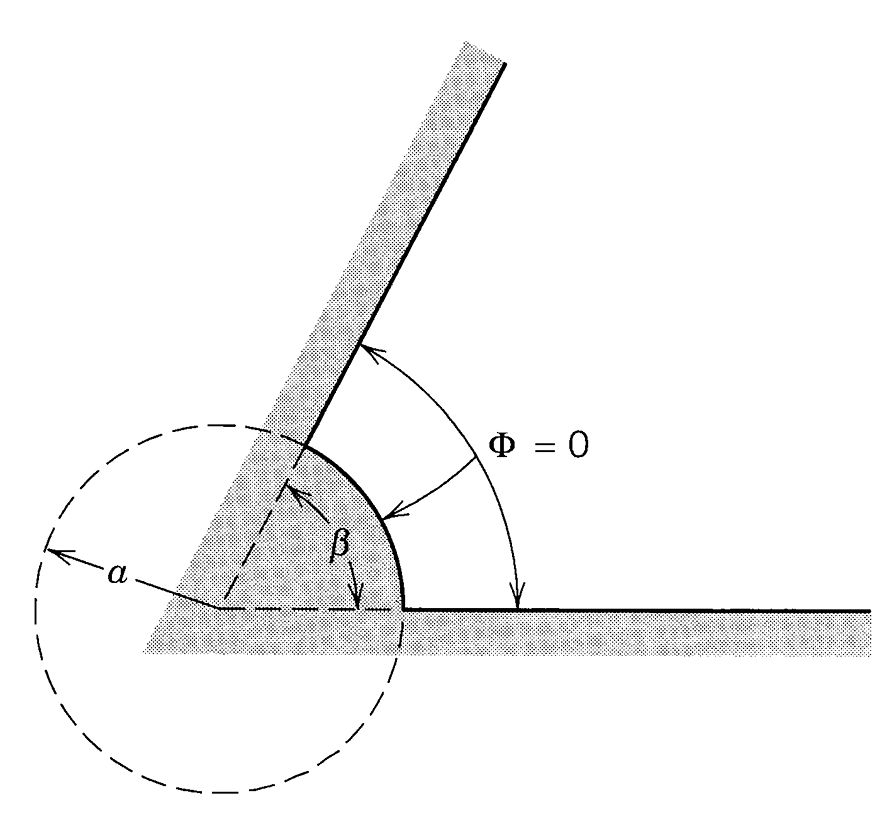
\includegraphics[width=0.5\textwidth]{hw4_p2.jpg}
\end{figure}

(a) Write down a solution for the potential $\Phi(\rho,\phi)$ that satisfies the
boundary conditions for finite $\rho$.

(b) Keeping only the lowest nonvanishing terms, calculate the electric field
components $E_\rho$ and $E_\phi$ and also the surface charge densities
$\sigma(\rho,0),\sigma(\rho,\beta)$, and $\sigma(a,\phi)$ on the three boundary
surfaces.

(c) Consider $\beta=\pi$ (a plane conductor with a half-cylinder of radius $a$
on it). Show that far from the half-cylinder the lowest order terms of part (b)
give a uniform electric field normal to the plane. Sketch the charge density on
and in the neighborhood of the half-cylinder. For fixed electric field strength
far from the plane, show that the total charge on the half-cylinder (actually
charge per unit length in the $z$ direction) is twice as large as would reside
on a strip of width $2a$ in its absence. Show that the extra portion is drawn
from regions of the plane nearby, so that the total charge on a strip of width
large compared to $a$ is the same whether the half-cylinder is there or not.
\begin{solution}
(a) By separation of variable, we write $\Phi(\rho,\phi)=R(\rho)\Psi(\phi)$.
Similar to Section 2.11 in Jackson, the functions $R$ and $\Psi$ satisfy the
ordinary differential equations
\begin{equation}
    \frac{\rho}{R}\frac{d}{d\rho}\qty(\rho\frac{dR}{d\rho})=\nu^2
    \qquad\text{and}\qquad
    \frac1{\Psi}\frac{d^2\Psi}{d\phi^2}=-\nu^2
\end{equation}
If $\nu=0$, then the solutions are
\begin{equation}
    R_{\nu=0}(\rho)=A_0+B_0\ln\rho
    \qquad\text{and}\qquad
    \Psi_{\nu=0}(\phi)=C_0+D_0\phi
\end{equation}
However, the boundary conditions force these zeroth terms to vanish. At
$\phi=0$, $\Psi=C_0=0$ and $\phi=\beta\neq0$, $\Psi=D_0\beta=0$. So both $C_0$
and $D_0$ are zero. Now, for $\nu\neq 0$, the solutions are
\begin{subequations}
    \begin{align}
        R(\rho)&=A\rho^\nu+b\rho^{-\nu}\\
        \Psi(\phi)&=C\cos(\nu\phi)+D\sin(\nu\phi)
    \end{align} 
\end{subequations}
At $r=a$, $R=Aa^\nu+Ba^{-\nu}=0$, so $B=-Aa^{2\nu}$. At $\phi=0$, $\Psi=C=0$. At
$\phi=\beta$, $\Psi=D\sin(\nu\beta)=0$. Since the non-trivial solution has
$D\neq 0$, $\sin(\nu\beta)=0$ and thus $\nu=n\pi /\beta$ for $n\in\N$. Then we
can write the general solution for finite $\rho$ as
\begin{equation}
    \Phi(\rho,\phi)=\sum_{n\in\N}A_n\qty(\rho^{n\pi/\beta}-a^{2n\pi/\beta}\rho^{-n\pi/\beta})\sin\qty(\frac{n\pi\phi}{\beta}) 
\end{equation}

(b) The electric field is $\vb{E}=-\grad\Phi=-(\partial\Phi
/\partial\rho)\bm{\hat{\rho}}-(1 /\rho)(\partial\Phi /\partial\phi)\phihat$.
Thus, up to the first non-trivial term, the components are
\begin{equation}
    E_\rho=-\frac{\pi
    A_1}{\beta}\qty(\rho^{\pi/\beta-1}+a^{2\pi/\beta}\rho^{-\pi/\beta-1})\sin\qty(\frac{\pi\phi}{\beta}) 
\end{equation}
and
\begin{equation}
    E_\phi=-\frac{\pi
    A_1}{\beta}\qty(\rho^{\pi/\beta-1}-a^{2\pi/\beta}\rho^{-\pi/\beta-1})\cos\qty(\frac{\pi\phi}{\beta}) 
\end{equation}

Now, the surface-charge density is $\sigma=\epsilon_0\vb{E}\vdot\nhat$ at a
conductor. At $\phi=0$, $\nhat=\phihat$. Thus,
\begin{equation}\label{p2b:sig_rho1}
    \sigma(\rho,0)=\epsilon_0
    \eval{E_\phi}_{\phi=0}
    =-\frac{\pi\epsilon_0}{\beta}A_1\qty(\rho^{\pi/\beta-1}-a^{2\pi/\beta}\rho^{-\pi/\beta-1}) 
\end{equation}
Similarly, at $\phi=\beta$, $\nhat=-\phihat$ and we can write
\begin{equation}\label{p2b:sig_rho2}
    \sigma(\rho,\beta)=
    -\epsilon_0\eval{E_\phi}_{\phi=\beta}
    =-\frac{\pi\epsilon_0}{\beta}A_1\qty(\rho^{\pi/\beta-1}-a^{2\pi/\beta}\rho^{-\pi/\beta-1}) 
\end{equation}
At $\rho=a$, $\nhat=\bm{\hat\rho}$, so
\begin{equation}\label{p2b:sig_phi}
    \sigma(a,\phi)=\epsilon_0E_\rho
    =-\frac{2\pi\epsilon_0}{\beta}A_1a^{\pi/\beta-1}\sin\qty(\frac{\pi\phi}{\beta})
\end{equation}

(c) At $\beta=\pi$, the electric field components are
\begin{subequations}
    \begin{align}
        E_\rho&=-A_1\qty[1+\qty(\frac{a}{\rho})^2]\sin\phi\\ 
        E_\phi&=-A_1\qty[1-\qty(\frac{a}{\rho})^2]\cos\phi
    \end{align} 
\end{subequations}
We can now write the electric field in Cartesian coordinates
\begin{align}
    \vb{E}&=E_\rho\bm{\hat\rho}+E_\phi\phihat\notag\\
          &=E_\rho(\cos\phi\xhat+\sin\phi\yhat)+E_\phi(-\sin\phi\xhat+\cos\phi\yhat)\notag\\
          &=\qty(E_\rho\cos\phi-E_\phi\sin\phi)\xhat
          +\qty(E_\rho\sin\phi+E_\phi\cos\phi)\yhat\notag\\
          &=-2A_1\sin\phi\cos\phi\qty(\frac{a}{\rho})^2\xhat
          -A_1\qty[1+\qty(\frac{a}{\rho})^2(\sin^2\phi-\cos^2\phi)]\yhat
\end{align}
So for $\rho\to\infty$, $E_x\to 0$ and $E_y\to -A_1$. The electric field is thus
uniform in the direction normal to the plane ($\yhat$). The charge densities
\eqref{p2b:sig_rho1}, \eqref{p2b:sig_rho2}, and \eqref{p2b:sig_phi} are now
simplified to
\begin{subequations}
    \begin{align}
        \sigma(\rho,0)&=-\epsilon_0A_1\qty[1-\qty(\frac{a}{\rho})^2]\label{p2c:sig_rho1}\\ 
        \sigma(\rho,\beta)&=-\epsilon_0A_1\qty[1-\qty(\frac{a}{\rho})^2]\label{p2c:sig_rho2}\\ 
        \sigma(a,\phi)&=-2\epsilon_0A_1\sin\phi\label{p2c:sig_cyl}
    \end{align} 
\end{subequations}
Note that $-\epsilon_0A_1=\epsilon_0E_\infty=\sigma_0$ is the charge density of
an infinite plane conductor. A plot of these charge densities is given below.
The top panel shows the density on the half-cylindrical surface, while the
bottom panel shows the density near the cylinder ($\rho\gtrsim a$ and
$\rho\lesssim-a$).
\begin{center}
    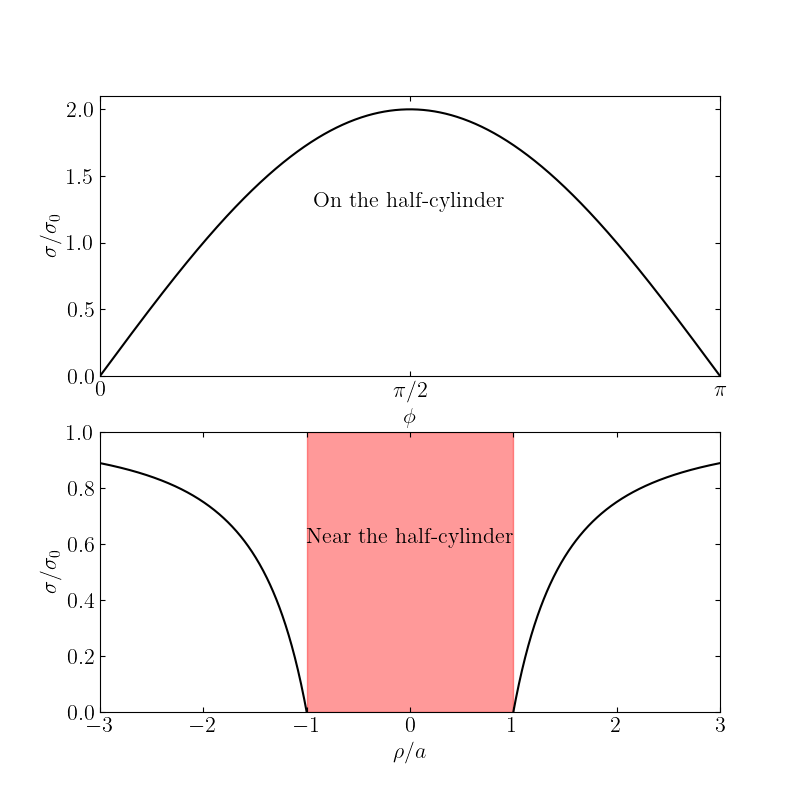
\includegraphics[width=0.8\textwidth]{p2.png}
\end{center}
From \eqref{p2c:sig_cyl}, the total charge on the half-cylinder is
\begin{align}
    Q_{cyl}=\int\sigma da=2a\sigma_0\int_0^\pi\sin\phi
    d\phi\int_0^zdz'=4a\sigma_0z
\end{align}
Thus, the charge per unit length in $z$ is
\begin{equation}\label{p2c:q_cyl}
    q_{cyl}=\frac{Q_{cyl}}{z}=4a\sigma_0 
\end{equation}
If there were no half-cylinder, the surface charge density would be $\sigma_0$.
So the total charge per unit length $z$ on the strip from $-a$ to $a$ is
\begin{equation}\label{p2c:strip}
    q_{strip}=\sigma_0\int_{-a}^adx=2a\sigma_0 
\end{equation}
Thus, $q_{cyl}=2q_{strip}$. Now, we integrate for the charge near the
half-cylinder. Because of the symmetry in \eqref{p2c:sig_rho1} and
\eqref{p2c:sig_rho2}, we know that the charge in the positive $\rho$ region
$q_+$ is the same as the charge in the negative $\rho$ region $q_-$. Thus, we
need only calculate $q_+$ from $a$ to $L$ where $L>a$
\begin{equation}
    q_+\approx\sigma_0\int_a^Ldx=\sigma_0(L-a)=q_- 
\end{equation}
The total charge including those on the half-cylinder and those near it is
\begin{equation}
    q_{total}=q_{cyl}+2q_+=2\sigma_0(L+a)=2\sigma_0L\qty(1+\frac{a}{L}) 
\end{equation}
If $L\gg a$, then $q_{total}=2\sigma_0L$. However, if there were no cylinder,
the charge of the strip would be $q_{strip}=2\sigma_0L$, as indicated by 
\eqref{p2c:strip}. This means the extra charge calculated in \eqref{p2c:q_cyl}
that leads to $q_{cyl}=2q_{strip}$ is drawn from regions of the plane nearby.
\end{solution}
\end{problem}
%%%%%%%%%%%%%%%%%%%%%%%%%%%%%%%%%%%%%%%%%%%%%%%%%%%%%%%%%%%%%%%%%%%%%%%%%%%%%%%%    
%%%%%%%%%%%%%%%%%%%%%%%%%%%%%%%%%%%%%%%%%%%%%%%%%%%%%%%%%%%%%%%%%%%%%%%%%%%%%%%%
\begin{problem}{3.3}[A sphere with a hole in the top]
A spherical surface of radius $R$ has charge uniformly distributed over its
surface with a density $Q /4\pi R^2$, except for a spherical cap at the north
pole, defined by the cone $\theta=\alpha$.

(a) Show that the potential inside the spherical surface can be expressed as
\begin{equation}
    \Phi=\frac{Q}{8\pi\epsilon_0}\sum_{l=0}^\infty\frac{r^l}{R^{l+1}}\frac{P_{l+1}(\cos\alpha)-P_{l-1}(\cos\alpha)}{2l+1}P_l(\cos\theta) 
\end{equation}
where, for $l=0,P_{l-1}(\cos\alpha)=-1$. What is the potential inside?

(b) Find the magnitude and the direction of the electric field at the origin.

(c) Discuss the limiting forms of the potential (part a) and electric field
(part b) as the spherical cap becomes (1) very small, and (2) so large that the
area with charge on it becomes a very small cap at the south pole.
\begin{solution}
(a) This problem has an azimuthal symmetry, so the potential can be generally
written as
\begin{equation}
    \Phi(r,\theta)=\sum_{l=0}^\infty\qty(A_lr^l+B_lr^{-(l+1)})P_l(\cos\theta) 
\end{equation}
Inside the sphere, $r^{-(l+1)}$ blows up at $r=0$, so $B_l=0$ for all $l$.
Similarly, outside the sphere, $A_l=0$ because $r^l\to\infty$ at large radius.
Then we have the solution inside and outside the sphere as
\begin{subequations}
    \begin{align}
        \Phi_{in}&=\sum_{l=0}^\infty A_lr^lP_l(\cos\theta) \\
        \Phi_{out}&=\sum_{l=0}^\infty B_lr^{-(l+1)}P_l(\cos\theta) 
    \end{align}
\end{subequations}
By continuity, $\eval{\Phi_{in}}_{r=R}=\eval{\Phi_{out}}_{r=R}\Rightarrow
B_l=A_lR^{2l+1}$. Also, we can calculate the surface charge density at $r=R$
from the potential inside and outside the sphere
\begin{align}
    \sigma&=-\epsilon_0\qty[
        \eval{\frac{\partial\Phi_{out}}{\partial r}}_{r=R}
        -\eval{\frac{\partial\Phi_{in}}{\partial r}}_{r=R}
    ]\notag\\
    &=-\epsilon_0\sum_{l=0}^\infty
        \qty[-(l+1)B_lr^{-(l+2)}-lA_lR^{l-1}]P_l(\cos\theta)\notag\\
    &=\epsilon_0\sum_{l=0}^\infty A_l(2l+1)R^{l-1}P_l(\cos\theta)
\end{align}
Now, we are also given the surface charge density
\begin{equation}
    \sigma(\theta)=\begin{cases}
        \frac{Q}{4\pi R^2} & \theta>\alpha\\
        0 & \theta\leq\alpha
    \end{cases}
\end{equation}
Thus, for $\theta>\alpha$ we can find the coefficients $A_l$ by using the
orthogonality condition
\begin{align}
    A_l(2l+1)R^{l-1}=\frac{2l+1}{2}\int_{\alpha}^\pi
    \sigma(\theta)P_l(\cos\theta)\sin\theta d\theta 
    =\frac{Q}{4\pi\epsilon_0 R^2}\frac{2l+1}{2}\int_{\alpha}^\pi
    P_l(\cos\theta)\sin\theta d\theta
\end{align}
Thus,
\begin{equation}
    A_l=\frac{Q}{8\pi\epsilon_0}R^{-(l+1)}\frac{P_{l+1}(\cos\alpha)-P_{l-1}(\cos\alpha)}{2l+1} 
\end{equation}
Then we can write the solution for $\Phi$ as
\begin{subequations}
    \begin{align}
        \Phi_{in}&=\frac{Q}{8\pi\epsilon_0}\sum_{l=0}^\infty
            \frac{r^l}{R^{l+1}}\frac{P_{l+1}(\cos\alpha)-P_{l-1}(\cos\alpha)}
                {2l+1}P_l(\cos\theta)\\
        \Phi_{out}&=\frac{Q}{8\pi\epsilon_0}\sum_{l=0}^\infty
            \frac{R^l}{r^{l+1}}\frac{P_{l+1}(\cos\alpha)-P_{l-1}(\cos\alpha)}
            {2l+1}P_l(\cos\theta)\label{p3:P_out}
    \end{align} 
\end{subequations}

Note that for $r\gg R$, the potential should be approximately that of a point
charge
\begin{equation}\label{p3:P_inf}
    \Phi_\infty\approx\frac{1}{4\pi\epsilon_0}\frac{1}{r}\int\sigma da
    =\frac1{4\pi\epsilon_0}\frac1r\frac{Q}{2}\int_{\alpha}^\pi\sin\theta
    d\theta
    =\frac{Q(\cos\alpha+1)}{8\pi\epsilon_0r}
\end{equation}
From \eqref{p3:P_out},
\begin{align}\label{p3:P_out_inf}
    \Phi_{out}=\frac{Q}{8\pi\epsilon_0}\frac1r\qty[\cos\alpha-P_{-1}(\cos\alpha)]+\order{r^{-2}}\approx\frac{Q(\cos\alpha-P_{-1}(\cos\alpha))}{8\pi\epsilon_0
    r}
\end{align}
Comparing \eqref{p3:P_inf} and \eqref{p3:P_out_inf}, we must then require that
$P_{-1}(\cos\alpha)=-1$.

(b) The electric field is $\vb{E}=-\grad\Phi=-(\partial\Phi /\partial r)\rhat-(1
/r)(\partial\Phi /\partial\theta)\thetahat$. In the radial direction,
\begin{align}
    E_r&=
    -\frac{Q}{8\pi\epsilon_0}\frac{\partial}{\partial r}\qty[
        \frac{\cos\alpha+1}{R}+\sum_{l=1}^\infty\frac{r^l}{R^{l+1}}\frac{P_{l+1}(\cos\alpha)-P_{l-1}(\cos\alpha)}{2l+1}P_l(\cos\theta)
    ]\notag\\
       &=-\frac{Q}{8\pi\epsilon_0}\sum_{l=1}^\infty l\frac{r^{l-1}}{R^{l+1}}
        \frac{P_{l+1}(\cos\alpha)-P_{l-1}(\cos\alpha)}{2l+1}P_l(\cos\theta)\notag\\
       &=-\frac{Q}{8\pi\epsilon_0}\qty[
        -\frac{\sin^2\alpha}{2R^2}\cos\theta+\sum_{l=2}^\infty
            l\frac{r^{l-1}}{R^{l+1}}\frac{P_{l+1}(\cos\alpha)-P_{l-1}(\cos\alpha)}{2l+1}P_l(\cos\theta)
       ]
\end{align}
Thus, $E_r(r=0)=(Q /16\pi\epsilon_0R^2)\sin^2\alpha\cos\theta$. In the polar
direction,
\begin{align}
    E_\theta&=-\frac{Q}{8\pi\epsilon_0 r}\frac{\partial}{\partial\theta}
    \qty[
    \frac{\cos\alpha+1}{R}+\sum_{l=1}^\infty\frac{r^l}{R^{l+1}}\frac{P_{l+1}(\cos\alpha)-P_{l-1}(\cos\alpha)}{2l+1}P_l(\cos\theta)
    ]\notag\\
    &=-\frac{Q}{8\pi\epsilon_0}\sum_{l=1}^\infty\frac{r^{l-1}}{R^{l+1}}\frac{P_{l+1}(\cos\alpha)-P_{l-1}(\cos\alpha)}{2l+1}\frac{l\cos\theta
    P_{l}(\cos\theta)-lP_{l-1}(\cos\theta)}{\sin\theta}\tag{from (3.29,
Jackson)}\\
    &=-\frac{Q}{8\pi\epsilon_0}\frac{\sin^2\alpha}{2R^2}\sin\theta
    -\frac{Q}{8\pi\epsilon_0}\sum_{l=2}^\infty
        \frac{r^{l-1}}{R^{l+1}}\frac{P_{l+1}(\cos\alpha)-P_{l-1}(\cos\alpha)}{2l+1}\frac{l\cos\theta
    P_{l}(\cos\theta)-lP_{l-1}(\cos\theta)}{\sin\theta}
\end{align}
Thus, $E_\theta(r=0)=-(Q /16\pi\epsilon_0R^2)\sin^2\alpha\sin\theta$. Putting
these results together, we can write the electric field as
\begin{equation}\label{p3b:E}
    \vb{E}(r=0)=\frac{Q}{16\pi\epsilon_0}\frac{\sin^2\alpha}{R^2}\qty(\cos\theta\rhat-\sin\theta\thetahat)=\frac{Q}{16\pi\epsilon_0}\frac{\sin^2\alpha}{R^2}\zhat
\end{equation}

(c) First, from \eqref{p3b:E}, whenever $\alpha\ll 1$,
$\sin\alpha\approx\alpha$ and we can write
\begin{equation}
    \vb{E}=\frac{Q}{16\pi\epsilon_0}\frac{\alpha^2}{R^2}\zhat 
\end{equation}
So $\vb{E}\to\vb{0}$ as $\alpha\to 0$. This is the case of a closed conductor,
and we know that the electric field in a hollow conductor must be zero. Now, in
the other limit, let $\beta=\pi-\alpha$ and consider $\beta\ll 1$. Since
$\sin\alpha=\sin(\pi-\beta)=\sin\beta$, $\vb{E}\to\vb{0}$ when $\beta\to 0$.
Now, this makes sense because the total charge on the sphere is
$Q(\cos\alpha+1) /2=Q(1-\cos\beta) /2\to 0$ when $\beta\to 0$.

Now, the potential inside the sphere is
\begin{align}
    \Phi_{in}
    &=\frac{Q}{8\pi\epsilon_0}\sum_{l=0}^\infty\frac{r^l}{R^{l+1}}\frac{P_{l+1}(\cos\alpha)-P_{l-1}(\cos\alpha)}{2l+1}P_l(\cos\theta)\notag\\
    &=\frac{Q}{8\pi\epsilon_0}\qty[\frac{\cos\alpha+1}{R}
    +\sum_{l=1}^\infty\frac{r^l}{R^{l+1}}\frac{P_{l+1}(\cos\alpha)-P_{l-1}(\cos\alpha)}{2l+1}P_l(\cos\theta)
    ]\notag\\
    &=\frac{Q}{8\pi\epsilon_0}\qty[\frac{\cos\alpha+1}{R}+\order{\alpha^2}]
\end{align}
As $\alpha\to 0$, to first order, $\Phi_{in}$ approaches the potential of the 
sphere at $r=R$. We know that $\vb{E}=\vb{0}$ in this case, so $\Phi_{in}$ is a 
constant. Because it has to satisfy the continuity with the outside potential, 
this is the expected result. In the other limit $\beta=\pi-\alpha\to 0$,
$\cos\alpha=-\cos\beta$, so $\Phi_{in}\to 0$ for the same reason as the 
vanishing of the electric field (total charge $\to 0$).

Similarly, the potential outside the sphere is
\begin{align}
    \Phi_{out}
    &=\frac{Q}{8\pi\epsilon_0}\sum_{l=0}^\infty
        \frac{R^l}{r^{l+1}}\frac{P_{l+1}(\cos\alpha)-P_{l-1}(\cos\alpha)}{2l+1}
            P_l(\cos\theta)\notag\\
    &=\frac{Q}{8\pi\epsilon_0}\qty[\frac{\cos\alpha+1}{r}
        +\order{\alpha^2}
    ]
\end{align}
As $\alpha\to 0$, this approachs the potential of a conducting sphere with
charge $Q$
\begin{equation}
    \Phi_{out}\to\frac{Q}{4\pi\epsilon_0 r} 
\end{equation}
as expected. In the opposite limit, $\beta\to 0$ and $\Phi_{out}\to 0$, because
the total charge decreases as in the other cases.
\end{solution}
\end{problem}
%%%%%%%%%%%%%%%%%%%%%%%%%%%%%%%%%%%%%%%%%%%%%%%%%%%%%%%%%%%%%%%%%%%%%%%%%%%%%%%%    
%%%%%%%%%%%%%%%%%%%%%%%%%%%%%%%%%%%%%%%%%%%%%%%%%%%%%%%%%%%%%%%%%%%%%%%%%%%%%%%%
\begin{problem}{4.4}[Conducting disc]

A thin, flat, conducting, circular disc of radius $R$ is located in the $xy$
plane with its center at the origin, and is maintained at a fixed potential $V$.
With the information that the charge density on a disc at fixed potential is
proportional to $(R^2-\rho^2)^{-1 /2}$, where $\rho$ is the distance out from
the center of the disc,

(a) show that for $r>R$ the potential is
\begin{equation}
    \Phi(r,\theta,\phi)=\frac{2V}{\pi}\frac{R}{r}\sum_{l=0}^\infty\frac{(-1)^l}{2l+1}\qty(\frac{R}{r})^{2l}P_{2l}(\cos\theta) 
\end{equation}

(b) find the potential for $r<R$.

(c) What is the capacitance of the disc?
\begin{solution}
(a) Given a surface charge density $\sigma=\alpha /\sqrt{R^2-\rho^2}$ where
$\rho$ is the radius in cylindrical coordinates and $\alpha$ is some constant, 
we can integrate to find the charge of an infinitesimally thin ring
\begin{equation}
    q_{ring}=\int_0^{2\pi}\sigma\rho d\rho d\phi=2\pi\alpha\frac{\rho
    d\rho}{\sqrt{R^2-\rho^2}} 
\end{equation}
In Section 3.3 of Jackson, the potential contribution (at $\vb{x}=r\zhat$ with 
$r<R$) of a thin ring placed at $b=0$ is
\begin{equation}
    d\Phi=\frac{\alpha}{2\epsilon_0}\frac{\rho
    d\rho}{\sqrt{R^2-\rho^2}}\sum_{l=0}^\infty\frac{r^l}{\rho^{l+1}}P_l(0) 
\end{equation}
Then we can integrate for the total potential
\begin{align}
    \Phi
    =\frac{\alpha}{2\epsilon_0}\sum_{l=0}^\infty\qty(\int_0^R\frac{d\rho}{\sqrt{R^2-\rho^2}\rho^l})r^lP_l(0)
=\frac{\alpha}{2\epsilon_0}\qty[\int_0^R\frac{d\rho}{\sqrt{R^2-\rho^2}}+C(r)]
\end{align}
where $C(r)=C_1r+C_2r^2+\ldots$ is a polynomial in $r$. At $r=0$, $C(r)=0$ and
\begin{equation}
    \Phi=\frac{\pi\alpha}{4\epsilon_0}=V\Rightarrow\alpha=\frac{4\epsilon_0V}{\pi}
\end{equation}
for some fixed value $V$.

For $r>R$, the potential contribution by a thin ring is
\begin{equation}
    d\Phi=\frac{2V}{\pi}\sum_{l=0}^\infty\frac{\rho^{l+1}d\rho}{\sqrt{R^2-\rho^2}}\frac{P_l(0)}{r^{l+1}}=\frac{2V}{\pi}\sum_{l=0}^\infty\frac{\rho^{2l+1}d\rho}{\sqrt{R^2-\rho^2}}\frac{P_{2l}(0)}{r^{2l+1}}
\end{equation}
where we have used the fact that $P_l(0)$ is only non-zero for some even $l$.
Then, we can integrate for the total potential
\begin{align}\label{p4a:Phi}
    \Phi&=\frac{2V}{\pi}\sum_{l=0}^\infty\qty(\int_0^R\frac{\rho^{2l+1}d\rho}{\sqrt{R^2-\rho^2}})\frac{P_{2l}(0)}{r^{2l+1}}
    \notag\\
        &=\frac{2V}{\pi}\sum_{l=0}^\infty\frac{\sqrt\pi}{2}\frac{\Gamma(l+1)}{\Gamma(l+3/2)}\qty(\frac{R}{r})^{2l+1}P_{2l}(0)
\end{align}
where $\Gamma(l)=(l-1)!$ is the Gamma function. Now, we also know that
\begin{equation}
    P_{2l}(0)=\frac{(-1)^l(2l)!}{2^{2l}(l!)^2} 
\end{equation}
Plugging this into \eqref{p4a:Phi} results in
\begin{align}\label{p4a:Phi2}
    \Phi&=\frac{2V}{\pi}\frac{R}{r}\sum_{l=0}^\infty\frac{\sqrt\pi}{2}\frac{l!}{(l+1/2)!}\frac{(-1)^l(2l)!}{2^{2l}(l!)^2}\notag\\
        &=\frac{2V}{\pi}\frac{R}{r}\sum_{l=0}^\infty\frac{(-1)^l(2l)!}{(2l+1)!}\qty(\frac{R}{r})^{2l}\notag\\
        &=\frac{2V}{\pi}\frac{R}{r}\sum_{l=0}^\infty\frac{(-1)^l}{2l+1}\qty(\frac{R}{r})^{2l}
\end{align}
where we have used $l!(l+1 /2)! =\sqrt{\pi}2^{-1-2l}(2l+1)!$ in the second
equality. \eqref{p4a:Phi2} is the solution on the $z$ axis. So for every point
in space,
\begin{equation}
    \Phi(r,\theta)=\frac{2V}{\pi}\frac{R}{r}\sum_{l=0}^\infty\qty(\frac{R}{r})^{2l}\frac{(-1)^l}{2l+1}P_{2l}(\cos\theta) 
\end{equation}
due to azimuthal symmetry.

(c) The total charge on the disc is
\begin{equation}
    Q=\int_0^R\sigma \rho d\rho\int_0^{2\pi}d\phi=2\pi\alpha\int_0^R\frac{\rho
    d\rho}{\sqrt{R^2-\rho^2}}=8\epsilon_0 VR 
\end{equation}
Thus, the capacitance is $C=Q /V=8\epsilon_0R$.
\end{solution}
\end{problem}
%%%%%%%%%%%%%%%%%%%%%%%%%%%%%%%%%%%%%%%%%%%%%%%%%%%%%%%%%%%%%%%%%%%%%%%%%%%%%%%%
\end{document}
